\documentclass[11pt]{article}

\usepackage[margin=1in]{geometry}
\usepackage{graphicx}
\usepackage{booktabs}
\usepackage{array}
\usepackage{float}
\usepackage{xcolor}
\usepackage{hyperref}
\usepackage{amsmath}
\usepackage{amssymb}
\usepackage{siunitx}
\usepackage{enumitem}

\graphicspath{{figures/}{docs/figures/}}
\hypersetup{
  colorlinks=true,
  linkcolor=blue!55!black,
  urlcolor=blue!55!black,
  citecolor=blue!55!black
}
\setlist[itemize]{topsep=3pt,itemsep=2pt,parsep=0pt}
\setlist[enumerate]{topsep=3pt,itemsep=2pt,parsep=0pt}
\sisetup{round-mode=places,round-precision=3}

\title{\textbf{DroneRace Training Report}\\
\large PPO Training Strategy, Adaptive Entropy, Reward Design, and In-Progress Results}
\author{EECS106B DroneRace Project}
\date{Snapshot from active run ending near 369.6M frames}

\begin{document}
\maketitle

\begin{abstract}
This report documents the current DroneRace reinforcement-learning approach in
the working tree. The task trains an Iris quadrotor to fly an ordered 13-gate
race track in Isaac Sim using PPO. The current method is intentionally
accuracy-first: the agent is rewarded primarily for crossing gates in order, and
speed pressure is delayed until full-lap completion is reliable. This document
explains the environment, observations, control interface, PPO loop, adaptive
entropy schedule, reward and curriculum choices, current training behavior, and
the most important risks and next steps. The included plots are generated from
the in-progress log
\texttt{.logs/DroneRace-rewardfix-12h-simple-2048-20260419-162107.log}. Since
the run was still active when inspected, all results should be read as a
point-in-time training snapshot.
\end{abstract}

\section{Scope and Source of Truth}

This report describes the current implementation, not an idealized algorithm.
The working tree is treated as the source of truth. The main files are listed in
Table~\ref{tab:sources}.

\begin{table}[H]
\centering
\caption{Primary source files for the current DroneRace training setup.}
\label{tab:sources}
\small
\begin{tabular}{p{0.43\linewidth}p{0.48\linewidth}}
\toprule
\textbf{File} & \textbf{Role} \\
\midrule
\path{omni_drones/envs/drone_race/drone_race.py} &
Environment, observations, gate crossing, rewards, termination, curriculum
stats. \\
\path{cfg/task/DroneRace.yaml} &
Track layout, environment count, episode length, reward scales, crash
thresholds. \\
\path{cfg/algo/DroneRace.yaml} &
PPO hyperparameters, actor/critic widths, privileged inputs, adaptive entropy
settings. \\
\path{scripts/train.py} &
Hydra config merge, data collection, W\&B logging, adaptive entropy update,
checkpointing. \\
\path{omni_drones/learning/ppo/ppo.py} &
PPO actor/critic implementation, GAE, value normalization, clipped objective. \\
\bottomrule
\end{tabular}
\end{table}

The existing README contains some stale language about an older four-gate
diamond track. This report uses the current YAML and Python implementation
instead: the active task is a 13-gate track with elevated gates and
same-position vertical reversal sections.

\section{Environment and Track}

The task trains one Iris quadrotor per environment. The drone is controlled by a
rate controller, while PPO learns the higher-level rate and thrust commands.
The configured track contains 13 gate entries:

\begin{itemize}
  \item YAML gates 1--12 form the real ordered course.
  \item YAML gate 13 duplicates YAML gate 1 and closes the lap.
  \item YAML gates 7 and 11 are elevated gates.
  \item Gates 7 $\rightarrow$ 8 and 11 $\rightarrow$ 12 share the same XY
  positions but differ in height and facing direction. These are the hardest
  local maneuvers in the course.
\end{itemize}

The episode and simulation settings are summarized in
Table~\ref{tab:env-settings}.

\begin{table}[H]
\centering
\caption{Environment and simulation settings.}
\label{tab:env-settings}
\begin{tabular}{lll}
\toprule
\textbf{Setting} & \textbf{Value} & \textbf{Purpose} \\
\midrule
\texttt{sim.dt} & 0.002 & Physics integration timestep. \\
\texttt{sim.substeps} & 5 & PPO action applied every 5 physics steps. \\
Policy rate & \SI{100}{Hz} & High-rate control for racing maneuvers. \\
\texttt{max\_episode\_length} & 2000 steps & 20 seconds per episode. \\
Default \texttt{num\_envs} & 512 & Stable default training throughput. \\
Active-run \texttt{num\_envs} & 2048 & Higher-throughput override in current run. \\
\texttt{train\_every} & 256 & 2.56 seconds of rollout per env per PPO batch. \\
\bottomrule
\end{tabular}
\end{table}

The track design is not just a navigation problem; it is also a sequence
problem. Passing a later gate does not help unless the current target gate is
crossed first. This is why the environment tracks a per-environment
\texttt{gate\_indices} tensor and only advances the target when the current gate
is crossed in the correct direction and inside the aperture.

\section{Observation and Control Interface}

\subsection{Observation Vector}

The actor receives a compact 33-dimensional observation. Absolute world position
is not included. Instead, the policy receives local gate geometry and vehicle
state, which is more directly relevant to racing control.

\begin{table}[H]
\centering
\caption{Actor observation components.}
\label{tab:obs}
\small
\begin{tabular}{p{0.37\linewidth}cp{0.43\linewidth}}
\toprule
\textbf{Component} & \textbf{Dim.} & \textbf{Reason} \\
\midrule
Body-frame linear velocity & 3 & Forward/lateral/vertical motion in the drone frame. \\
Rotation matrix & 9 & Orientation without quaternion sign ambiguity. \\
Angular velocity & 3 & Stabilization and body-rate awareness. \\
Previous action & 4 & Helps learn smooth, history-aware control. \\
Distance to gate center & 1 & Gives the norm directly. \\
Current gate relative position, drone frame & 3 & Main navigation vector. \\
Next-to-next gate vector & 3 & Lookahead for turns and reversals. \\
Current gate orientation columns & 6 & Encodes gate facing and lateral axis. \\
Normalized gate index & 1 & Course-position signal for gate-specific maneuvers. \\
\bottomrule
\end{tabular}
\end{table}

The gate-relative observation points to the gate center, not the gate asset
origin. This matters because the gate asset origin is at the bottom center. The
environment adds \(\texttt{gate\_height}/2\) in the gate frame so that
observation, reward, and crossing detection all refer to the same aperture
center.

\subsection{Action Space and Controller}

The policy emits a 4D action:

\begin{equation}
a_t =
\begin{bmatrix}
\omega_x^\star & \omega_y^\star & \omega_z^\star & T^\star
\end{bmatrix}.
\end{equation}

The first three dimensions are target body-rate commands and the final
dimension is target thrust. Before execution, actions are clamped to
\([-1,1]\). The rate controller maps the clamped command into rotor commands.

This choice avoids forcing PPO to learn low-level motor mixing. It also keeps
the policy close to the control abstraction used in practical agile flight:
learn where to point and how hard to thrust, while the controller tracks rates.
The main tradeoff is that the PPO actor samples from an unbounded Gaussian, but
the simulator executes the clamped action. Therefore the log probability used
for PPO is not always the probability of the exact executed command. This
mismatch is most relevant when entropy is high and many sampled actions saturate.

\section{PPO Training Algorithm}

\subsection{Data Collection and Update Schedule}

The active run uses 2048 vectorized environments and
\(\texttt{train\_every}=256\). Each PPO update therefore consumes

\begin{equation}
2048 \times 256 = 524{,}288
\end{equation}

new environment frames. With the default 512 environments, the same rollout
length would produce 131,072 frames per update.

\begin{table}[H]
\centering
\caption{Active-run PPO batch structure.}
\label{tab:ppo-batch}
\begin{tabular}{lr}
\toprule
\textbf{Quantity} & \textbf{Value} \\
\midrule
Parallel environments & 2048 \\
Rollout length & 256 steps \\
Frames per PPO update & 524,288 \\
PPO epochs & 10 \\
Minibatches per epoch & 16 \\
Samples per minibatch & 32,768 \\
Gradient updates per rollout & 160 \\
\bottomrule
\end{tabular}
\end{table}

The 256-step rollout length is deliberate. At \SI{100}{Hz}, it covers
\SI{2.56}{s} per environment, long enough to include meaningful gate approach
and crossing events once the policy begins moving through the track.

\subsection{Policy and Value Networks}

The actor and critic are MLPs with layer normalization and LeakyReLU
activations. The actor outputs the mean and standard deviation of an independent
normal distribution. The critic predicts a scalar value. Both actor and critic
receive privileged intrinsics in the current configuration.

\begin{table}[H]
\centering
\caption{Network and optimizer configuration.}
\label{tab:networks}
\begin{tabular}{ll}
\toprule
\textbf{Item} & \textbf{Configuration} \\
\midrule
Actor hidden units & \texttt{[256, 256]} \\
Critic hidden units & \texttt{[256, 256, 128]} \\
Activation & \texttt{leaky\_relu} \\
Layer normalization & Enabled \\
Actor learning rate & \(3\times 10^{-4}\) \\
Critic learning rate & \(3\times 10^{-4}\) \\
Optimizer & Adam \\
Gradient clipping & 5.0 \\
Critic loss & Huber, \(\delta = 10.0\) \\
\bottomrule
\end{tabular}
\end{table}

The wider critic is a reasonable choice because value estimation is harder than
action selection in this sparse/semisparse task. The critic also benefits more
from privileged physical parameters.

\subsection{Objective, GAE, and Value Normalization}

The PPO update uses the clipped surrogate objective:

\begin{align}
r_t(\theta) &=
\exp\left(\log \pi_\theta(a_t|s_t) -
          \log \pi_{\theta_{\mathrm{old}}}(a_t|s_t)\right), \\
L_{\mathrm{actor}} &=
-\mathbb{E}\left[
\min\left(
r_t(\theta) A_t,
\mathrm{clip}(r_t(\theta), 1-\epsilon, 1+\epsilon) A_t
\right)\right].
\end{align}

The clip parameter is \(\epsilon=0.2\). Advantages are computed with GAE using
\(\gamma=0.998\) and \(\lambda=0.95\). The high discount factor is appropriate
because lap completion and later gate rewards are delayed relative to the
early-step control choices.

Returns are normalized by \texttt{ValueNorm1} before critic training. This is
useful because the return scale changes significantly during training: early
policies may crash or hover, while later policies collect hundreds of points
from ordered gate rewards.

One implementation caveat is important for future full-lap learning: the PPO
GAE mask currently uses \texttt{next/terminated}. In DroneRace,
\texttt{terminated} corresponds to crash termination, while timeout and
successful lap completion are represented through \texttt{done} and
\texttt{truncated}. Once lap completions appear, successful terminal
transitions should be masked for value bootstrap as well.

\section{Adaptive Entropy}

Entropy is the main exploration pressure in PPO. The policy loss includes

\begin{equation}
L_{\mathrm{entropy}} = -\alpha H(\pi_\theta(\cdot|s_t)),
\end{equation}

where \(\alpha\) is \texttt{entropy\_coef}. Minimizing this term encourages a
broader action distribution. A large coefficient improves exploration but can
make execution noisy; a small coefficient improves exploitation but can lock in
suboptimal behavior.

Although \texttt{cfg/algo/DroneRace.yaml} contains
\texttt{entropy\_coef: 0.001}, adaptive entropy is enabled, so
\texttt{scripts/train.py} updates the coefficient during training.

\begin{table}[H]
\centering
\caption{Adaptive entropy schedule.}
\label{tab:entropy}
\begin{tabular}{lll}
\toprule
\textbf{Parameter} & \textbf{Value} & \textbf{Role} \\
\midrule
\texttt{phase0\_coef\_max} & 0.012 & Maximum exploration before full laps exist. \\
\texttt{phase0\_coef\_min} & 0.002 & Lower phase-0 entropy near unlock accuracy. \\
\texttt{phase1\_rebump\_coef} & 0.010 & Exploration rebump when speed phase starts. \\
\texttt{phase1\_coef\_min} & 0.0005 & Low-entropy mature speed policy. \\
\texttt{speed\_ema\_alpha} & 0.05 & Smoothing for speed-performance signal. \\
\texttt{speed\_signal\_low} & 0.05 & Low gates-per-second baseline. \\
\texttt{speed\_signal\_high} & 0.60 & High gates-per-second target. \\
\texttt{max\_delta\_per\_update} & 0.0005 & Slew-rate limit for coefficient changes. \\
\bottomrule
\end{tabular}
\end{table}

In phase 0, the target entropy coefficient is reduced as the lap-completion EMA
approaches the speed-unlock threshold:

\begin{equation}
\alpha_{\mathrm{target}} =
\alpha_{\max}
- \frac{\mathrm{accuracy\_EMA}}{\mathrm{unlock\_rate}}
  (\alpha_{\max}-\alpha_{\min}).
\end{equation}

In phase 1, entropy is first rebumped. This is intentional: when the objective
changes from accurate completion to faster completion, a previously accurate
but slow policy may need fresh exploration to discover faster racing lines. Once
phase 1 is active, the coefficient decays with a smoothed gates-per-second
signal.

Figure~\ref{fig:entropy} shows the current state: the run remains in phase 0,
lap accuracy EMA is zero, and entropy remains at the phase-0 maximum.

\begin{figure}[H]
\centering
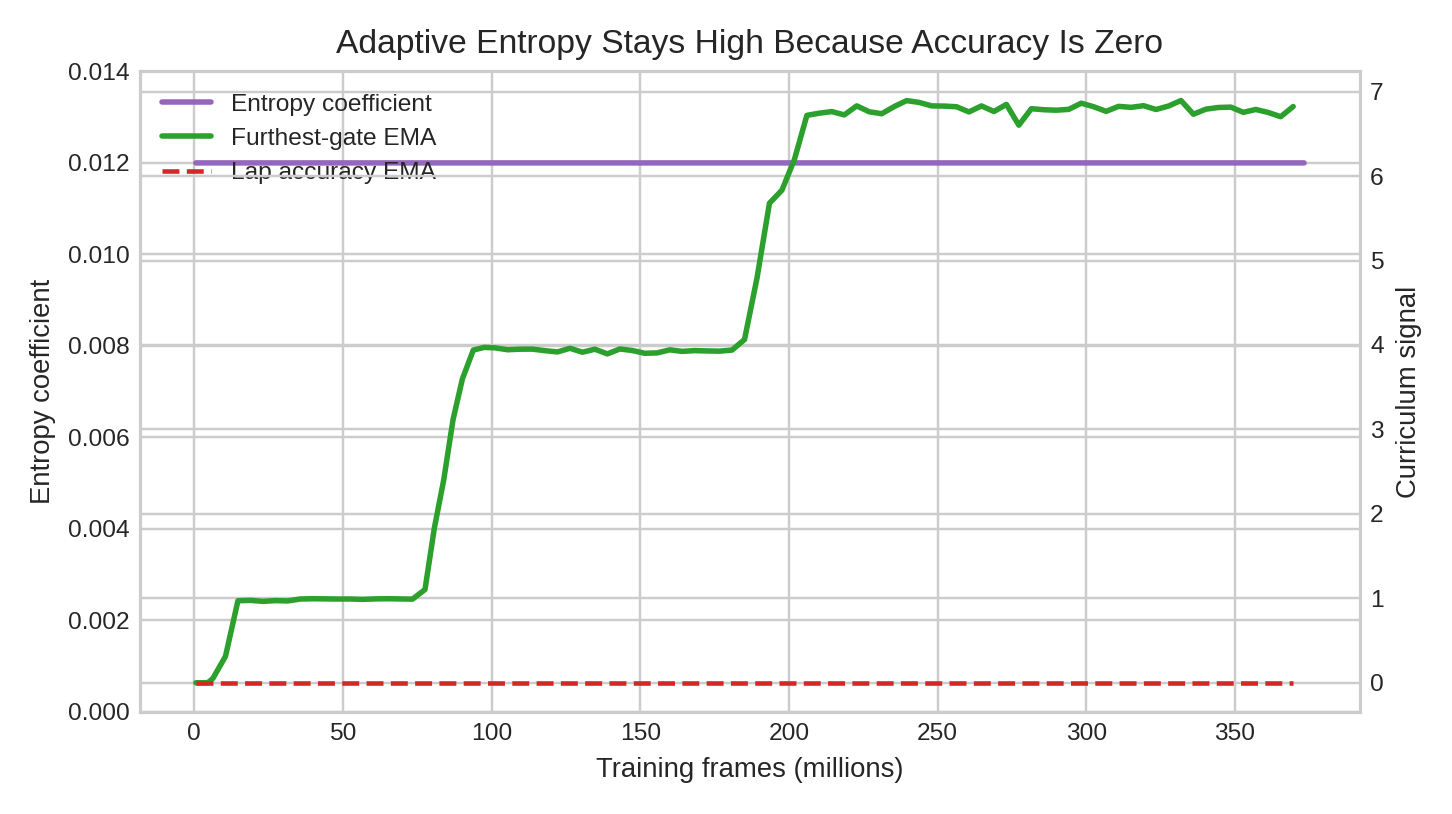
\includegraphics[width=0.9\linewidth]{drone_race_entropy_curriculum.png}
\caption{Adaptive entropy and curriculum signals. Entropy remains high because
full-lap accuracy has not yet appeared.}
\label{fig:entropy}
\end{figure}

\section{Reward and Curriculum Design}

\subsection{Reward Terms}

The reward is designed so that correct ordered gate passage dominates early
learning. Dense progress shaping is present, but intentionally small.

\begin{table}[H]
\centering
\caption{Positive reward terms.}
\label{tab:positive-rewards}
\begin{tabular}{lll}
\toprule
\textbf{Term} & \textbf{Scale} & \textbf{Purpose} \\
\midrule
Path-projection progress & 1.0 & Dense guidance along the current segment. \\
Gate passage & 60.0 & Sparse reward for crossing the target gate. \\
Ordered sequence & \(20.0 \times\) streak & Larger reward for longer ordered chains. \\
Lap completion & 500.0 & Makes finishing the full course primary. \\
Lap speed bonus & up to 300.0 & Rewards earlier completion after phase unlock. \\
\bottomrule
\end{tabular}
\end{table}

The path-projection reward projects the drone displacement onto the unit vector
from the previous gate center to the current target gate center. This provides
smooth local guidance but is not large enough to dominate the true objective.
The current scale of 1.0 is a deliberate correction: larger dense progress can
reward fly-bys that move along the course direction without passing through the
gate.

\begin{table}[H]
\centering
\caption{Penalty terms.}
\label{tab:penalties}
\small
\begin{tabular}{p{0.32\linewidth}p{0.16\linewidth}p{0.40\linewidth}}
\toprule
\textbf{Term} & \textbf{Scale} & \textbf{Purpose} \\
\midrule
Elevated-gate altitude mismatch & 0.5 & Encourages matching high gate centers. \\
Near-gate retreat & 0.5 & Penalizes backing away once close. \\
Gate-centering miss & 0.03 & Discourages near-plane fly-bys. \\
Angular-rate penalty & 0.1, decaying & Stabilizes early learning. \\
Action smoothness & 0.002 & Reduces abrupt actuator changes. \\
Crash penalty & 80.0 & Penalizes collision, ground, and divergence failures. \\
\bottomrule
\end{tabular}
\end{table}

The centering penalty is especially important. It only activates near the target
gate plane and uses lateral/vertical error in the gate frame. This reduces the
chance that the policy learns to skim past gates while still collecting dense
progress reward.

\subsection{Curriculum}

The curriculum has two phases:

\begin{itemize}
  \item \textbf{Phase 0:} accuracy-first ordered-lap learning from gate 0.
  \item \textbf{Phase 1:} speed-shaping after reliable full-lap completion.
\end{itemize}

The transition condition is:

\begin{equation}
\texttt{frames\_in\_phase} \ge 2{,}000{,}000
\quad \mathrm{and} \quad
\texttt{lap\_completion\_rate\_ema} \ge 0.40.
\end{equation}

The active run easily satisfies the frame floor, but the lap-completion EMA is
still zero. Therefore, phase 1 has not unlocked. This is the intended behavior:
speed pressure should not start before the policy can finish the course.

\subsection{Termination and Crash Logic}

Episodes end on success, timeout, or crash:

\begin{itemize}
  \item Success: the ordered lap is completed.
  \item Timeout: \texttt{progress\_buf >= max\_episode\_length}.
  \item Physical crash: base-link contact force is detected.
  \item Ground crash: altitude drops below \texttt{crash\_z\_min}.
  \item Distance crash: the drone diverges too far from the target gate.
\end{itemize}

Distance crash is disabled for a 100-step grace window after spawn or gate
crossing. Without this grace period, the target-gate jump after a successful
crossing could immediately make the next gate appear far away and falsely end
the episode.

\section{Training Results So Far}

This section keeps only the plots that explain the training state. The omitted
speed/crash plot was useful for sanity checking, but it is not the central
story: speed is already nontrivial and distance crashes are zero. The decisive
signals are course progress, the per-gate bottleneck, reward balance, and the
entropy/curriculum plot shown earlier in Figure~\ref{fig:entropy}.

The figures below were generated from the active log. The parser found 98
complete training-stat blocks. The latest complete parsed block was:

\begin{itemize}
  \item Epoch: 705
  \item Frames: 369,623,040
  \item Return: 945.29
  \item Gates passed per episode: 6.81
  \item Lap completion rate: 0.0
  \item Mean speed: \SI{3.93}{m/s}
  \item Total crash rate: 8.1\%
  \item Distance crash rate: 0.0\%
\end{itemize}

The data says that the agent is not stuck at takeoff or first-gate discovery.
It has learned a repeatable partial course. The failure is localized: the policy
clears the early track and usually reaches the first elevated section, but it
does not learn the same-XY drop/reversal immediately after that section.

\subsection{Course Progress}

Figure~\ref{fig:course-progress} shows that the policy has learned meaningful
ordered progress through the early track but has not yet completed laps. The
furthest-gate and gates-passed curves rise into the first elevated section and
then flatten around 6--7 gates. This plateau is the first high-level sign that
more global PPO updates are producing diminishing returns under the current
reset distribution.

\begin{figure}[H]
\centering
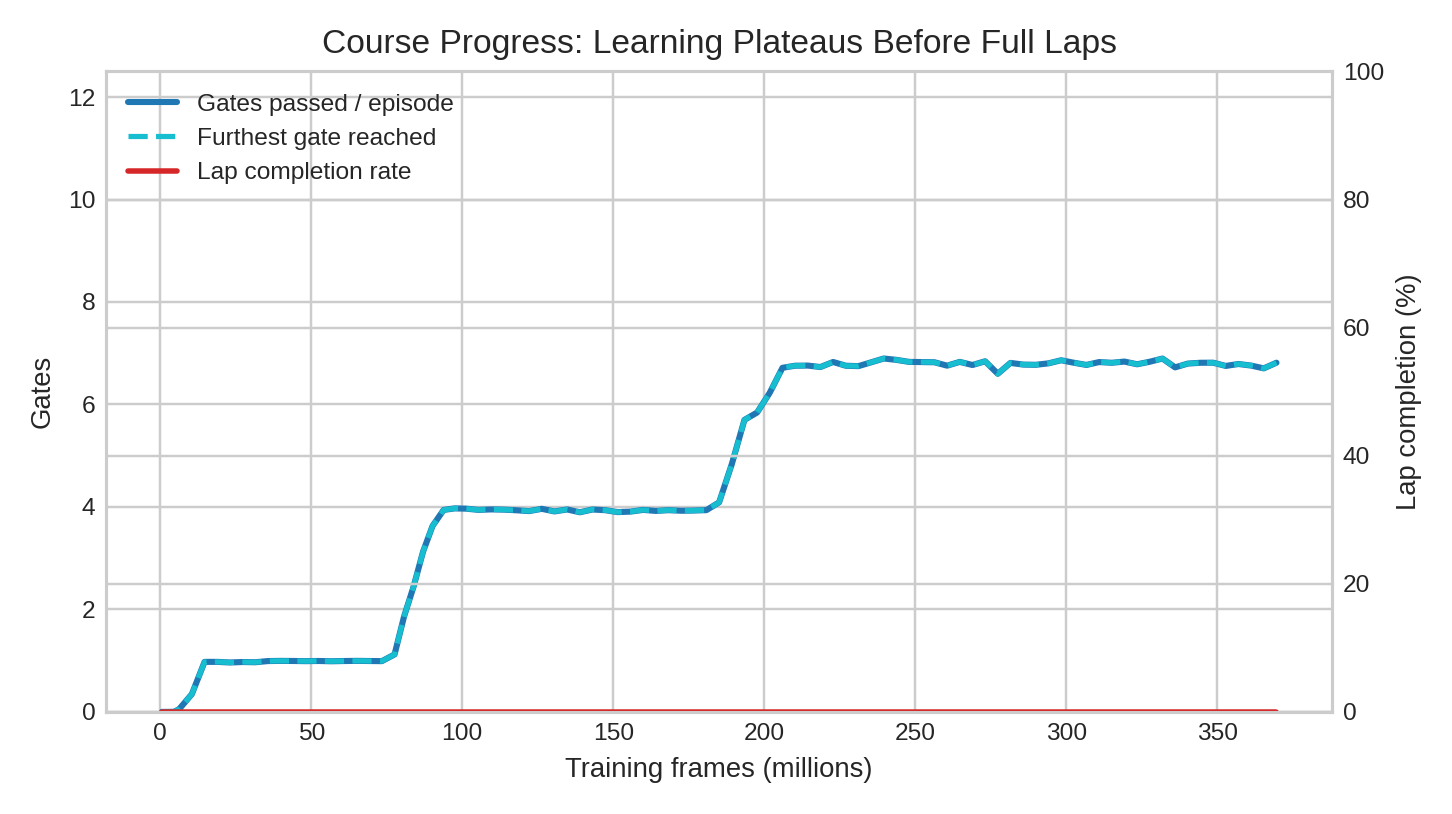
\includegraphics[width=0.92\linewidth]{drone_race_course_progress.png}
\caption{Course progress over training. The policy averages about 6.8 gates per
episode, but full-lap completion remains zero. The learning curve has plateaued
before the second half of the course.}
\label{fig:course-progress}
\end{figure}

\subsection{Per-Gate Bottleneck}

The per-gate crossing distribution in Figure~\ref{fig:gate-crossings} is the
most diagnostic plot. Crossings are near-reliable through zero-based gate 6.
Zero-based gate 6 corresponds to YAML gate 7, the first elevated gate. Crossing
rates collapse immediately after that. In the latest parsed block,
\texttt{gate\_06\_crosses}=0.939, while
\texttt{gate\_07\_crosses}=0.0 and all later gate crossings are 0.0.

\begin{figure}[H]
\centering
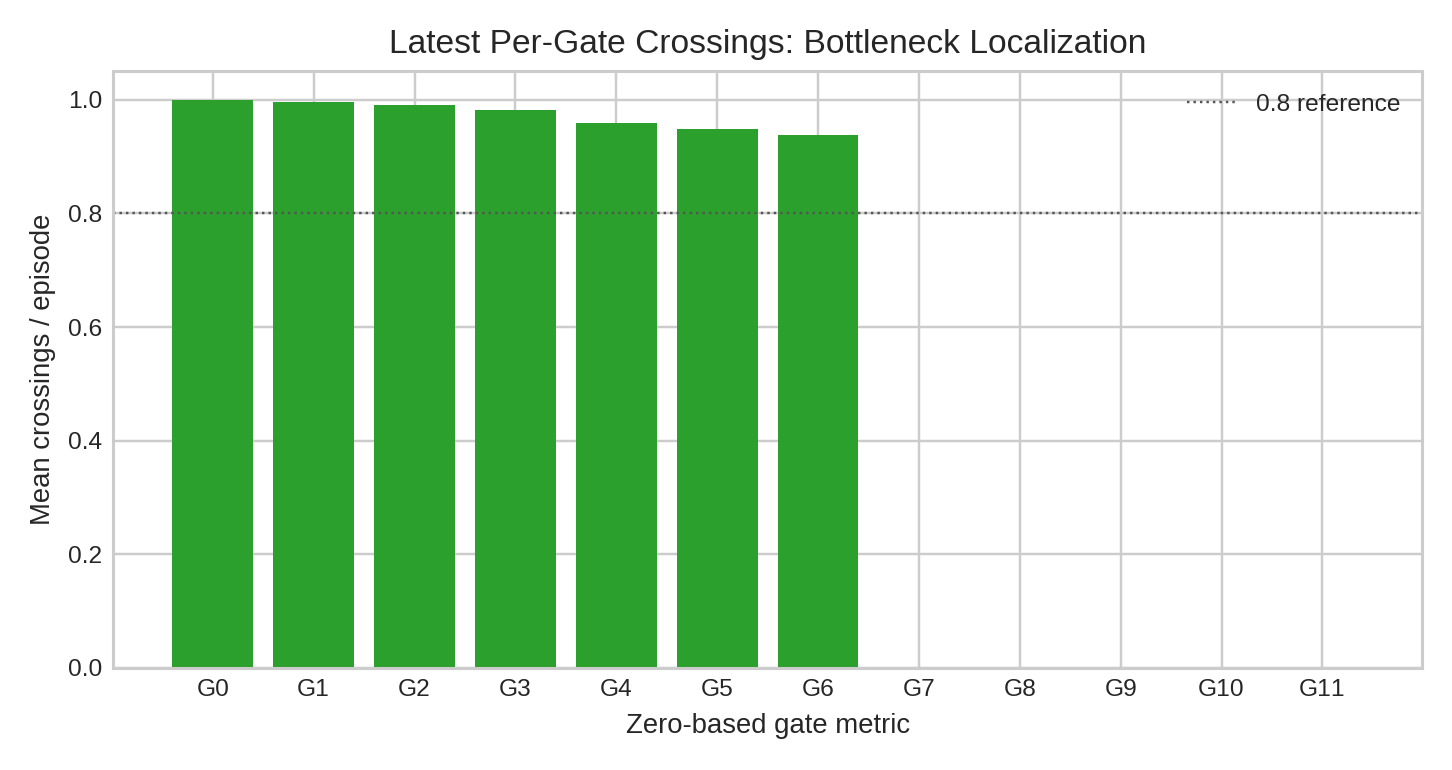
\includegraphics[width=0.92\linewidth]{drone_race_gate_crossings_latest.png}
\caption{Latest per-gate crossing distribution. The current bottleneck is the
transition after the first elevated gate, around YAML gates 7--8.}
\label{fig:gate-crossings}
\end{figure}

This indicates that the main failure is not generic early navigation. The policy
has learned the beginning of the course. The hard case is the same-XY
drop/reversal after the elevated gate. Because phase-0 resets always start at
gate 0, the policy receives many training samples on gates 0--6 and very few
successful or near-successful samples on gate 8. This explains why the run can
continue accumulating frames while the bottleneck remains nearly unchanged.

\subsection{Reward Balance}

Figure~\ref{fig:reward-components} shows that gate and sequence rewards dominate
return. This is intentional. The dense progress term is much smaller, and the
centering and altitude penalties remain bounded. The reward graph is important
because it rules out a common failure mode: the agent is not mainly earning
return from dense progress while ignoring gates. It is earning return from
ordered gate crossings.

\begin{figure}[H]
\centering
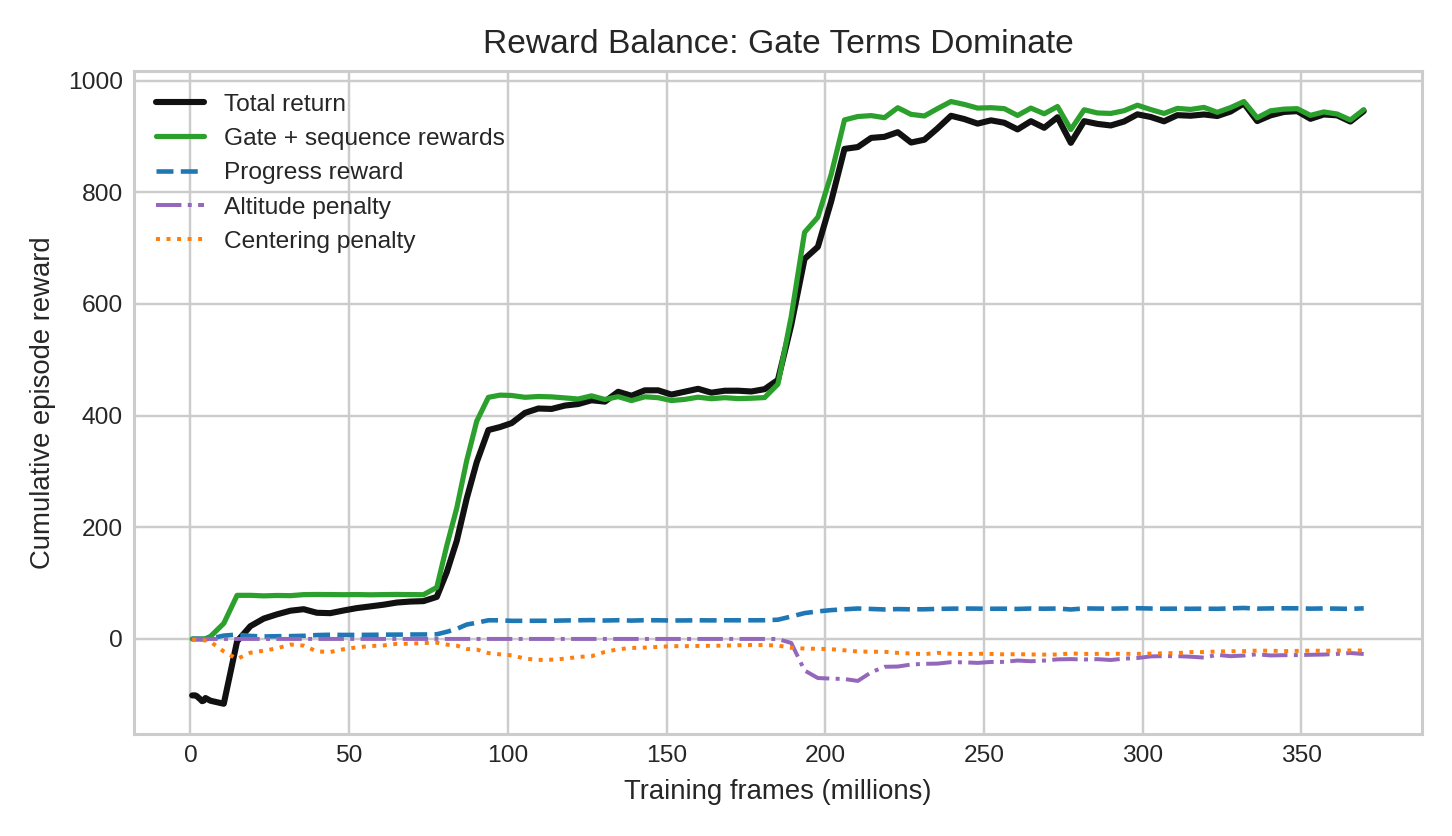
\includegraphics[width=0.92\linewidth]{drone_race_reward_components.png}
\caption{Reward components. Gate and sequence rewards dominate phase-0
learning, while dense progress remains a smaller guidance signal.}
\label{fig:reward-components}
\end{figure}

At the latest parsed block, reward components were approximately:

\begin{table}[H]
\centering
\caption{Latest parsed reward components.}
\label{tab:latest-reward}
\begin{tabular}{lr}
\toprule
\textbf{Metric} & \textbf{Value} \\
\midrule
\texttt{reward/total\_return} & 945.29 \\
\texttt{reward/gates\_cumul} & 947.93 \\
\texttt{reward/progress\_cumul} & 54.79 \\
\texttt{reward/altitude\_cumul} & -27.01 \\
\texttt{reward/approach\_cumul} & -3.06 \\
\texttt{reward/centering\_cumul} & -20.76 \\
\bottomrule
\end{tabular}
\end{table}

The reward balance matches the design intent: sparse ordered gate completion is
the dominant source of positive return. The progress term is only about 5.8\%
of total return in the latest block, while gate rewards are approximately equal
to the total positive return before penalties. That means the current plateau is
not caused by progress shaping overwhelming gate completion. It is more likely a
data-distribution and maneuver-specific issue.

\subsection{Interpretation of the Important Signals}

The four important signals form a consistent diagnosis:

\begin{enumerate}
  \item \textbf{Course progress has plateaued.} The policy reaches about 6.8
  gates per episode with zero lap completion. This means it has learned a
  partial route, not a full racing policy.

  \item \textbf{The per-gate plot localizes the failure.} Crossings are reliable
  through zero-based gate 6, then drop to zero. The bottleneck is therefore the
  first elevated-to-low reversal, not the early course.

  \item \textbf{Reward balance is healthy.} Gate rewards dominate; dense progress
  is small. The objective is mostly rewarding legal ordered gate passage, which
  is what we want in phase 0.

  \item \textbf{Adaptive entropy is behaving as designed.} The entropy
  coefficient remains at 0.012 because lap-completion EMA is 0.0. The algorithm
  is intentionally preserving exploration rather than prematurely exploiting an
  incomplete route.
\end{enumerate}

Supporting metrics agree with this interpretation. Mean speed is already near
\SI{3.93}{m/s}, max speed is near \SI{11.18}{m/s}, and distance crash rate is
0.0\%. Those numbers are useful sanity checks, but they do not explain the main
failure. The main failure is that the agent rarely receives useful practice on
the gate 7--8 maneuver under the current always-start-from-gate-0 curriculum.

\section{Novel and Distinctive Elements}

The approach should not be overclaimed as a new RL algorithm. It is PPO with
task-specific reward shaping and curriculum. However, several elements are
locally novel or distinctive for this project:

\begin{enumerate}
  \item \textbf{Accuracy-gated speed curriculum.} Speed pressure is withheld
  until full-lap completion EMA reaches a threshold. This reduces the common
  racing failure mode where the agent learns to move fast but not legally pass
  gates.

  \item \textbf{Adaptive entropy tied to curriculum state.} Entropy is high
  during phase-0 exploration, decays as full-lap accuracy improves, then rebumped
  when the objective changes to speed. This directly couples exploration to the
  task's learning stage instead of using a fixed entropy coefficient.

  \item \textbf{Gate-center consistency across observation, reward, and
  crossing detection.} The implementation corrects for the asset origin being
  at the bottom of the gate. This removes a subtle mismatch where the policy
  could aim at a different point than the crossing detector uses.

  \item \textbf{Lookahead without recurrence.} The next-to-next gate vector gives
  the policy limited racing-line anticipation while keeping the actor feedforward.

  \item \textbf{Per-gate crossing diagnostics as a first-class training signal.}
  The logged gate distribution makes bottlenecks immediately visible. In this
  run, it identifies the first elevated drop/reversal as the limiting maneuver.

  \item \textbf{Reward hierarchy that explicitly protects gate legality.}
  Dense path progress is kept small, while sparse ordered gate and sequence
  rewards dominate. The centering penalty further discourages fly-bys.
\end{enumerate}

The most important novelty is not any single reward term. It is the combination
of an accuracy-first curriculum, curriculum-aware entropy, gate-centered
geometry, and per-gate diagnostics. Together, these make the training process
more interpretable and less likely to optimize the wrong behavior.

\section{Limitations and Risks}

\begin{enumerate}
  \item \textbf{Hard-gate data scarcity.} Since phase 0 always starts behind
  gate 0, the policy gets many more samples on early gates than on gate 8. This
  slows learning at the first vertical reversal.

  \item \textbf{Clamped Gaussian mismatch.} PPO optimizes log probabilities of
  sampled Gaussian actions, but the simulator executes clamped actions. This is
  acceptable as a stabilizing patch but not mathematically ideal.

  \item \textbf{GAE terminal masking.} Successful lap completion should be
  treated as terminal for value bootstrap. The current mask uses crash
  termination and should be revisited before lap completions become common.

  \item \textbf{Endpoint gate crossing detection.} The current crossing detector
  checks previous/current gate-frame sign change and current aperture bounds. A
  segment-plane intersection would be more robust at high speed.

  \item \textbf{Privileged actor inputs.} The actor receives intrinsics. This is
  acceptable for sim-only fixed-vehicle performance, but it should be removed or
  limited to the critic for transfer-oriented experiments.
\end{enumerate}

\section{Recommended Next Steps}

\begin{enumerate}
  \item \textbf{Add targeted reset curriculum near gates 7--8 and 11--12.}
  Keep full-course training, but allocate some resets to the hard vertical
  reversal sections after early gates become reliable.

  \item \textbf{Implement segment-based gate crossing.} Intersect the drone's
  previous-current motion segment with the target gate plane, then check the
  intersection point against aperture bounds.

  \item \textbf{Add signed gate-frame shaping for reversal gates.} Reward
  progress in the current gate's crossing direction and penalize wrong-side
  approach near gates with reversed facing.

  \item \textbf{Use a bounded policy distribution.} A tanh-squashed Gaussian or
  equivalent bounded distribution would align PPO log probabilities with the
  executed action range.

  \item \textbf{Fix PPO done masking before full laps are common.} Include
  success and timeout semantics in the bootstrap mask used by GAE.

  \item \textbf{Keep the current reward hierarchy.} The latest results show that
  sparse ordered gate rewards are driving useful learning. The next bottleneck
  is local maneuver coverage, not global reward scale.
\end{enumerate}

\section{Conclusion}

The current DroneRace training system is a coherent PPO-based racing setup. Its
main design decision is to learn legal ordered gate completion before optimizing
speed. The in-progress run demonstrates meaningful learning: the policy
reliably clears early gates, reaches the first elevated section, and moves at
approximately \SI{4}{m/s} mean speed. However, it has not completed a lap. The
current bottleneck is localized at the first same-XY elevated-to-low reversal
after YAML gate 7.

The next improvements should therefore focus on the hard local transition:
targeted resets, more robust crossing detection, signed gate-frame shaping, and
eventual PPO action/discontinuity cleanup. These changes are more likely to
unlock full laps than simply increasing global training time with the same data
distribution.

\end{document}
